\section{Теоретична постановка}
\subsection{Системи за масово обслужване}

% Define global styles for Ti*k*Z diagrams
\tikzset{
	% GNode styles
	source/.style={circle, draw, minimum size=1cm, inner sep=0pt},
	queue/.style={rectangle, draw, minimum height=1cm, minimum width=2.5cm, inner sep=0pt, rounded corners=3pt},
	server/.style={rectangle, draw, minimum size=1cm, inner sep=0pt},
	sink/.style={circle, draw, minimum size=1cm, inner sep=0pt, path picture={
			\draw (path picture bounding box.south west) -- (path picture bounding box.north east);
			\draw (path picture bounding box.north west) -- (path picture bounding box.south east);
	}},
	dot/.style={circle, fill=black, minimum size=0.2cm, inner sep=0pt},
	% StateNode styles
	state/.style={circle, draw, minimum size=1.5cm},
	arrow/.style={-{Latex[width=2mm,length=2mm]}, thick},
	ratelabel/.style={midway, fill=white, inner sep=1pt}
}

Схематично, една система за масово обслужване с п паралелно работещи обслужващи устройства може да бъде представена чрез обобщената схема, показана на фиг.6.5.
	
	% ----------------------------------------------------------------------
	% Figure 6.5
	% ----------------------------------------------------------------------
	\begin{figure}[h]
		\centering
		\begin{tikzpicture}[node distance=1.5cm, auto]
			% Source
			\node [source] (g) {};
			\node [dot] at (g.center) {};
			\node [above=0.2cm of g] {G};
			
			% Queue
			\node [queue, right=of g] (qu) {};
			% Add the queue content (three empty circles and an arrow)
			\node [circle, draw, minimum size=0.5cm, xshift=-0.7cm] at (qu.center) {};
			\node [circle, draw, minimum size=0.5cm, xshift=0cm] at (qu.center) {};
			\node [circle, draw, minimum size=0.5cm, xshift=0.7cm] at (qu.center) {};
			\draw[arrow] (g) -- (qu.west);
			\node [above=0.2cm of qu] {QU};
			
			% Servers S1 to Sn
			\node [server, right=of qu.east, yshift=0.8cm] (s1) {};
			\node [dot] at (s1.center) {};
			\node [above=0.2cm of s1] {$S_1$};
			
			\node [right=of qu.east, yshift=-0.8cm] (sn) [server] {};
			\node [dot] at (sn.center) {};
			\node [below=0.2cm of sn] {$S_n$};
			
			% Connecting lines with arrows
			\draw[arrow] (qu.east) -| (s1.west);
			\draw[arrow] (qu.east) -| (sn.west);
			\draw[arrow] (g) -- (qu.west);
			
			% Sink
			\node [sink, right=of qu.east, xshift=1.5cm] (sink) {};
			
			% Connecting servers to sink
			\draw[arrow] (s1.east) -| (sink.west);
			\draw[arrow] (sn.east) -| (sink.west);
			
			% Dots in between servers
			\node [below=0.1cm of s1] {\vdots};
			
		\end{tikzpicture}
		\caption{Схема на система за масово обслужване: $G$ — източник на заявки, $QU$ — опашка, $S_1 \ldots S_n$ — обслужващи устройства}
		\label{fig:queue_scheme}
	\end{figure}
	
	% ----------------------------------------------------------------------
	% Document Text
	% ----------------------------------------------------------------------
	\noindent
	Нека да разгледаме система за масово обслужване, която има едно обслужващо устройство и 2 места за чакане в опашката. В случай, че и двете места за чакане са заети, то постъпилата заявка получава отказ за обслужване и напуска системата необслужена. В случай, че обслужващото устройство е заето и има свободно място в опашката, заявката застава на опашката и чака обслужване. Такава система има четири възможни състояния: $S_0$ — в системата няма заявки и обслужващото устройство е свободно; $S_1$ — в системата има една заявка и обслужващото устройство е заето; $S_2$ — в системата има две заявки, обслужващото устройство е заето и една заявка чака на опашка; $S_3$ — в системата има три заявки, обслужващото устройство е заето и две заявки чакат на опашка. Ако чрез $\lambda$ се означи интензивността на постъпващия поток от заявки, а чрез $\mu$ интензивността на обслужването на заявките, то графът на състоянията на системата ще има вида, показан на фиг.6.6.
	
	\vspace{1em}
	
	% ----------------------------------------------------------------------
	% Figure 6.6
	% ----------------------------------------------------------------------
	\begin{figure}[h]
		\centering
		\begin{tikzpicture}[node distance=2.5cm, auto]
			% Nodes
			\node [state] (s0) {$S_0$};
			\node [state, right=of s0] (s1) {$S_1$};
			\node [state, right=of s1] (s2) {$S_2$};
			\node [state, right=of s2] (s3) {$S_3$};
			
			% Forward arcs (lambda)
			\path[arrow] (s0) edge [bend left=50] node [ratelabel, above] {\(\lambda\)} (s1);
			\path[arrow] (s1) edge [bend left=50] node [ratelabel, above] {\(\lambda\)} (s2);
			\path[arrow] (s2) edge [bend left=50] node [ratelabel, above] {\(\lambda\)} (s3);
			
			% Backward arcs (mu)
			\path[arrow] (s1) edge [bend left=50] node [ratelabel, below] {\(\mu\)} (s0);
			\path[arrow] (s2) edge [bend left=50] node [ratelabel, below] {\(\mu\)} (s1);
			\path[arrow] (s3) edge [bend left=50] node [ratelabel, below] {\(\mu\)} (s2);
			
		\end{tikzpicture}
		\caption{Граф на състоянията на системата}
		\label{fig:state_graph}
	\end{figure}
	
	% ----------------------------------------------------------------------
	% Continued Text
	% ----------------------------------------------------------------------
	\noindent
	Както се вижда, постъпващият поток от заявки $\lambda$ увеличава номера на състоянието $S_i$ (броя на заявките в системата), а потокът на обслужванията $\mu$ го намалява. Подобни процеси се наричат \textbf{процеси на раждане и смърт} по аналогия с биологичните системи.
	
	Ако чрез $p_i$ се означат вероятностите на състоянията $S_i$, то използвайки правилото за съставяне на уравненията на Колмогоров се получава:
	\begin{equation}
		\begin{cases}
			\dot{p}_0 = -\lambda p_0 + \mu p_1 \\
			\dot{p}_1 = -(\lambda + \mu) p_1 + \mu p_2 + \lambda p_0 \\
			\dot{p}_2 = -(\lambda + \mu) p_2 + \mu p_3 + \lambda p_1 \\
			\dot{p}_3 = \lambda p_2 - \mu p_3
		\end{cases} \tag{6.9}
	\end{equation}
	
	с начални условия $p_i(0)$, които се пресмятат чрез нормиращото условие $p_0 + p_1 + p_2 + p_3 = 1$.
	
	Получените при решаването на системата (6.9) вероятности могат да се използват за определяне на следните обобщени характеристики на системата за масово обслужване - среден брой заявки в системата $L_s$ и средна дължина на опашката $L_q$:
	
	\begin{equation}
		L_s = \sum_{k=1}^{3} k p_k = p_1 + 2p_2 + 3p_3 \tag{6.10}
	\end{equation}
	
	\begin{equation}
		L_q = \sum_{k=2}^{3} (k-1) p_k = p_2 + 2p_3 \tag{6.11}
	\end{equation}
	
	Един друг важен параметър на всяка система за масово обслужване е вероятността за отказ от обслужване $p_{отк}$. За разглежданата система отказ настъпва когато опашката е пълна и обслужващото устройство е заето, следователно вероятността за отказ е равна на вероятността в системата да има три заявки, т.е $p_{отк} = p_3$.
	
	Симулаторът Vensim , начина за изграждане на моделите, тяхната редакция, настройка, анализ и визуализация на получените резултати са дадени тук:
	\href{https://drive.google.com/file/d/1KA7ELFZJiojeZf64hBvp-6mXSiMZjaoq/view?usp=sharing}{https://drive.google.com/file/d/1KA7ELFZJiojeZf64hBvp-6mXSiMZjaoq/view?usp=sharing}
	
	
\subsection{Задание за лабораторна работа}

\begin{enumerate}
	\item Да се определят характеристиките на системата с едно обслужващо устройство и две места за чакане при интензивност 10 бр/h, и производителност на устройството 126p/h, в началния момент от време в системата не е имало заявки, т.е. $p_0(0)=1, p_1(0)=p_2(0)=p_3(0)=0$.
	\item Да се сравнят получените резултати за системата от предишната точка чрез Vensim с получените аналитично. За целта може да се използва xls калкулатора и/или друго Windows приложение.
\end{enumerate}

\subsection{Аналитично решение}

При зададените параметри $\lambda = 10$ бр/h и $\mu = 12$ бр/h коефициентът на натоварване е:
\begin{equation}
	\rho = \frac{\lambda}{\mu} = \frac{10}{12} = \frac{5}{6} \approx 0{,}833 \tag{1}
\end{equation}

Тъй като $\rho \neq 1$, стационарните вероятности се пресмятат по формули (6.12) и (6.13) с $m = 2$:
\begin{equation}
	p_0 = \frac{1 - \rho}{1 - \rho^{m+2}} = \frac{1 - \tfrac{5}{6}}{1 - \left(\tfrac{5}{6}\right)^{4}}
	= \frac{\tfrac{1}{6}}{\tfrac{671}{1296}} = \frac{216}{671} \approx 0{,}3220 \tag{2}
\end{equation}
\begin{align*}
	p_1 &= \rho\, p_0 = \frac{180}{671} \approx 0{,}2683 \\
	p_2 &= \rho^2 p_0 = \frac{150}{671} \approx 0{,}2235 \\
	p_3 &= \rho^3 p_0 = \frac{125}{671} \approx 0{,}1863
\end{align*}

Проверка: $p_0 + p_1 + p_2 + p_3 = \dfrac{216 + 180 + 150 + 125}{671} = 1$ \checkmark

\vspace{0.5em}
Резултатите са обобщени в таблица~\ref{tab:steadystate}.

\begin{table}[h]
	\centering
	\caption{Стационарни вероятности на състоянията при $\lambda=10$~бр/h, $\mu=12$~бр/h}
	\label{tab:steadystate}
	\begin{tabular}{ccc}
		\toprule
		Състояние & Точна стойност & Приблизителна стойност \\
		\midrule
		$p_0$ & $216/671$ & $0{,}3220$ \\
		$p_1$ & $180/671$ & $0{,}2683$ \\
		$p_2$ & $150/671$ & $0{,}2235$ \\
		$p_3$ & $125/671$ & $0{,}1863$ \\
		\bottomrule
	\end{tabular}
\end{table}

Обобщените характеристики на системата се пресмятат по формули (6.10), (6.11), (6.14)--(6.16):

\begin{align*}
	p_{\text{отк}} &= p_3 = \frac{125}{671} \approx 0{,}1863 \\[4pt]
	f               &= 1 - p_3 = \frac{546}{671} \approx 0{,}8137 \\[4pt]
	L_q             &= p_2 + 2p_3 = \frac{150 + 250}{671} = \frac{400}{671} \approx 0{,}5961 \text{ бр.} \\[4pt]
	L_s             &= p_1 + 2p_2 + 3p_3 = \frac{180 + 300 + 375}{671} = \frac{855}{671} \approx 1{,}2742 \text{ бр.}
\end{align*}

Средното време за пребиваване на заявките се определя чрез \textbf{Закона на Литъл}.
Ефективният интензитет (заявките, които не получават отказ) е:
\begin{equation}
	\lambda_{\text{еф}} = \lambda (1 - p_{\text{отк}}) = 10 \cdot \frac{546}{671} \approx 8{,}137 \text{ бр/h} \tag{3}
\end{equation}

Оттук средните времена за престой са:
\begin{align*}
	W_s &= \frac{L_s}{\lambda_{\text{еф}}} = \frac{855}{5460} \approx 0{,}1566 \text{ h} \approx 9{,}4 \text{ мин} \\[4pt]
	W_q &= \frac{L_q}{\lambda_{\text{еф}}} = \frac{400}{5460} \approx 0{,}0733 \text{ h} \approx 4{,}4 \text{ мин}
\end{align*}

Резултатите показват, че при $\rho \approx 0{,}833$ системата работи с висока натовареност. Вероятността за отказ е $\approx 18{,}6\%$, средният брой заявки в системата е $L_s \approx 1{,}27$, а средното чакане в опашката е $W_q \approx 4{,}4$ мин.

\subsection{Сравнение с резултати от Vensim}

В таблицата е показан графичният модел, чрез който се извършва решаването на системата (6.9) при $\lambda=10$ бр/h, $\mu=12$ бр/h, в началния момент от време в системата не е имало заявки, т.е. $p_0(0)=1, \ p_1(0)=p_2(0)=p_3(0)=0$.

	% ----------------------------------------------------------------------
	% System Dynamics Graphical Model (Simplified TiKZ Representation)
	% ----------------------------------------------------------------------
	\begin{figure}[h]
		\centering
		\begin{tikzpicture}[node distance=2.5cm, auto, >=Latex]
			% Styles for System Dynamics
			\tikzset{
				stock/.style={rectangle, draw, minimum width=1.2cm, minimum height=0.8cm},
				src/.style={ellipse, draw, minimum width=0.8cm, minimum height=0.5cm}
			}
			% ... (rest of the code remains the same)
			
			% Blocks for P0 to P3
			\node [stock] (p0) at (4, -2)  {P0};
			\node [stock] (p1) at (4, -4)  {P1};
			\node [stock] (p2) at (4, -6)  {P2};
			\node [stock] (p3) at (4, -8)  {P3};

			\node [src] (c0) at (0, -2)  {};
			\node [src] (c1) at (0, -4)  {};
			\node [src] (c2) at (0, -6)  {};
			\node [src] (c3) at (0, -8)  {};

			\draw [double, ->, thick] (c0) -- node[pos=0.5, above] {P0dot} (p0);
			\draw [double, ->, thick] (c1) -- node[pos=0.5, above] {P1dot} (p1);
			\draw [double, ->, thick] (c2) -- node[pos=0.5, above] {P2dot} (p2);
			\draw [double, ->, thick] (c3) -- node[pos=0.5, above] {P3dot} (p3);

			% Auxiliaries for Ls and Lq
			\node [right=of p1, xshift=2cm, yshift=-0.5cm] (ls) {Ls};
			\node [right=of p3, xshift=2cm, yshift=0.5cm] (lq) {Lq};
			
			% Information arrows
			\draw [blue!60, ->] (p1) -- (ls);
			\draw [blue!60, ->] (p2) -- (ls);
			\draw [blue!60, ->] (p3) -- (ls);
			
			\draw [blue!60, ->] (p2) -- (lq);
			\draw [blue!60, ->] (p3) -- (lq);
		\end{tikzpicture}
	\end{figure}
	
	% ----------------------------------------------------------------------
	% Model Equations Table
	% ----------------------------------------------------------------------
	\begin{center}
		\begin{tabular}{|l l|}
			\hline
			(01) & FINAL TIME = 1 \\
			(02) & INITIAL TIME = 0 \\
			(03) & lambda = 10 \\
			(04) & Lq = P2 + 2 * P3 \\
			(05) & Ls = P1 + 2 * P2 + 3 * P3 \\
			(06) & mu = 12 \\
			(07) & P0 = INTEG(P0dot, 1) \\
			(08) & P0dot = -lambda * P0 + mu * P1 \\
			(09) & P1 = INTEG(P1dot, 0) \\
			(10) & P1dot = -(lambda + mu) * P1 + lambda * P0 + mu * P2 \\
			(11) & P2 = INTEG(P2dot, 0) \\
			(12) & P2dot = -(lambda + mu) * P2 + lambda * P1 + mu * P3 \\
			(13) & P3 = INTEG(P3dot, 0) \\
			(14) & P3dot = -mu * P3 + lambda * P2 \\
			(15) & SAVEPER = TIME STEP \\
			(16) & TIME STEP = 0.01 \\
			\hline
		\end{tabular}
	\end{center}
	
	% ----------------------------------------------------------------------
	% Figure 6.7: System Characteristics Plots
	% ----------------------------------------------------------------------
	\begin{figure}[h]
		\centering
		\begin{minipage}{0.48\textwidth}
			\centering
			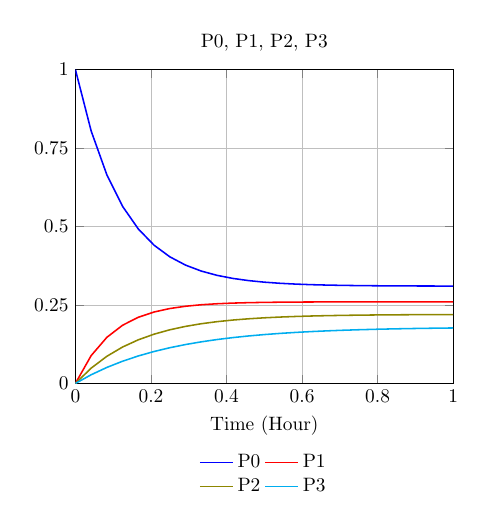
\begin{tikzpicture}[scale=0.7]
				\begin{axis}[
					title={P0, P1, P2, P3},
					xlabel={Time (Hour)},
					xmin=0, xmax=1,
					ymin=0, ymax=1,
					xtick={0, 0.20, 0.40, 0.60, 0.80, 1},
					ytick={0, .25, .5, .75, 1},
					grid=both,
					legend columns=2,
					legend style={at={(0.5,-0.2)}, anchor=north, draw=none}
					]
					% Qualitative representation of the transient state curves
					\addplot[blue, thick, domain=0:1] {0.31 + 0.69*exp(-8*x)}; 
					\addplot[red, thick, domain=0:1] {0.26*(1-exp(-10*x))};
					\addplot[olive, thick, domain=0:1] {0.22*(1-exp(-6*x))};
					\addplot[cyan, thick, domain=0:1] {0.18*(1-exp(-4*x))};
					\legend{P0, P1, P2, P3}
				\end{axis}
			\end{tikzpicture}
			\\ а)
		\end{minipage}
		\hfill
		\begin{minipage}{0.48\textwidth}
			\centering
			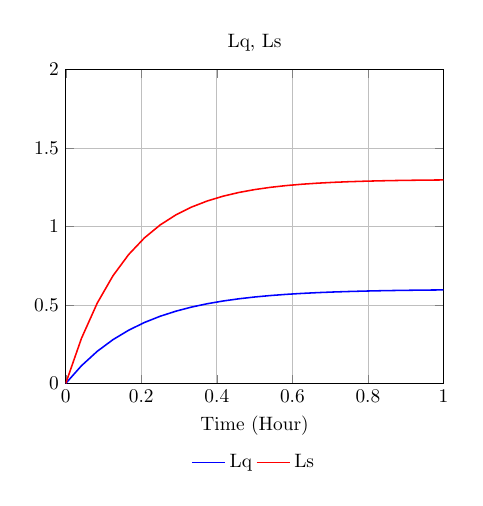
\begin{tikzpicture}[scale=0.7]
				\begin{axis}[
					title={Lq, Ls},
					xlabel={Time (Hour)},
					xmin=0, xmax=1,
					ymin=0, ymax=2,
					xtick={0, 0.20, 0.40, 0.60, 0.80, 1},
					ytick={0, 0.5, 1, 1.5, 2},
					grid=both,
					legend columns=2,
					legend style={at={(0.5,-0.2)}, anchor=north, draw=none}
					]
					\addplot[blue, thick, domain=0:1] {0.6*(1-exp(-5*x))};
					\addplot[red, thick, domain=0:1] {1.3*(1-exp(-6*x))};
					\legend{Lq, Ls}
				\end{axis}
			\end{tikzpicture}
			\\ б)
		\end{minipage}
		\caption{фиг.6.7 Характеристики на системата: а) вероятности на състоянията; б) обобщени характеристики на системата}
	\end{figure}
	
	% ----------------------------------------------------------------------
	% Steady State Equations
	% ----------------------------------------------------------------------
	\noindent Аналитичното изследване на разглежданата система показва, че вероятностните на състоянията на системата в стационарен режим могат да се пресметнат по следните формули:
	
	\begin{equation}
		p_0 = \frac{1 - \rho}{1 - \rho^{m+2}}, \text{ при } \rho \neq 1 \tag{6.12}
	\end{equation}
	
	\begin{equation}
		p_1 = \rho p_0, \ p_2 = \rho^2 p_0, \ \dots, \ p_m = \rho^m p_0, \ p_{m+1} = \rho^{m+1} p_0 \tag{6.13}
	\end{equation}
	
	Средният брой на заявките в опашката и системата се определя по следните зависимости:
	
	\begin{equation}
		L_q = \frac{\rho^2 (1 - \rho^m (m+1-m\rho))}{(1 - \rho^{m+2})(1 - \rho)} \tag{6.14}
	\end{equation}
	
	\begin{equation}
		f = 1 - p_3 \tag{6.15}
	\end{equation}
	
	\begin{equation}
		L_s = L_q + f \tag{6.16}
	\end{equation}
	
	\noindent където $\rho = \lambda / \mu$ се нарича \textbf{коефициент на натоварване на системата}, $f$ — среден брой на заявките, които се обслужват в обслужващите устройства (среден брой на заетите канали), $m$ е максималния възможен брой на заявките в опашката, в случая $m=2$.
	
	За определяне на средното време за пребиваване на заявките в системата се използва \textbf{Законът на Литъл}, който свързва средния брой заявки с интензивността и средното време на престой:

\begin{equation}
	L = \lambda_{\text{еф}} \cdot W \tag{6.17}
\end{equation}

\noindent където $\lambda_{\text{еф}} = \lambda (1 - p_{\text{отк}})$ е ефективният интензитет на постъпващите заявки (тези, които не получават отказ). Оттук средното време за пребиваване в системата $W_s$ и средното време на чакане в опашката $W_q$ са:

\begin{equation}
	W_s = \frac{L_s}{\lambda_{\text{еф}}} = \frac{L_s}{\lambda (1 - p_{\text{отк}})} \tag{6.18}
\end{equation}

\begin{equation}
	W_q = \frac{L_q}{\lambda_{\text{еф}}} = \frac{L_q}{\lambda (1 - p_{\text{отк}})} \tag{6.19}
\end{equation}

\noindent Очевидно е, че $W_s = W_q + \frac{1}{\mu}$, тъй като средното време за обслужване е $\frac{1}{\mu}$.
	